\documentclass[border=10pt]{standalone}
\usepackage{tikz}
\usetikzlibrary{calc}
\begin{document}
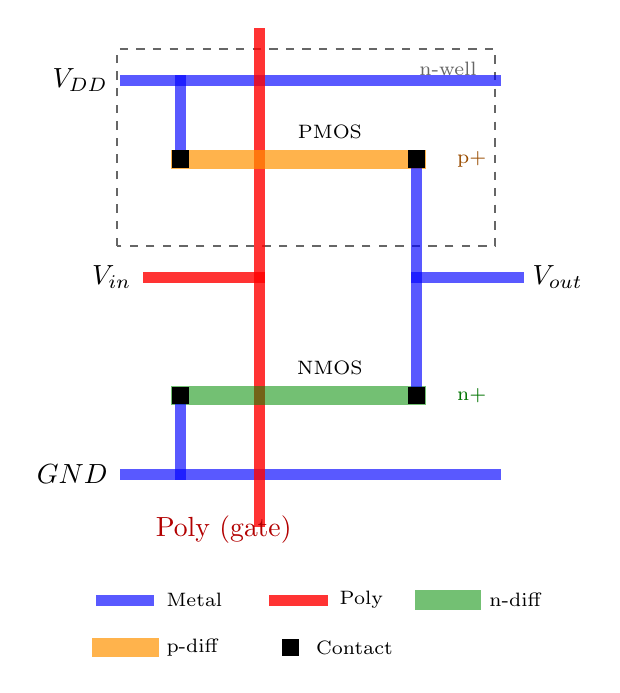
\begin{tikzpicture}[scale=1.0,
  metal/.style={blue, line width=4pt, line cap=rect, opacity=0.65},
  poly/.style={red, line width=4pt, line cap=rect, opacity=0.8},
  ndiff/.style={green!55!black, line width=7pt, line cap=rect, opacity=0.55},
  pdiff/.style={orange!85!yellow, line width=7pt, line cap=rect, opacity=0.7},
  contact/.style={draw=black, fill=black, minimum size=6pt, inner sep=0pt},
  nwell/.style={dashed, draw=black!60, line width=0.8pt}]

  % n-well around the PMOS region
  \draw[nwell] (0.2,2.9) rectangle (5.0,5.4);
  \node[black!60] at (4.4,5.15) {\scriptsize n-well};

  % VDD and GND metal rails
  \draw[metal] (0.3,5) -- (5,5);   \node[left] at (0.2,5) {$V_{DD}$};
  \draw[metal] (0.3,0) -- (5,0);   \node[left] at (0.2,0) {$GND$};

  % polysilicon gate (input), spans both transistors
  \draw[poly] (2,-0.6) -- (2,5.6);
  \node[red!70!black] at (1.55,-0.7) {Poly (gate)};
  \draw[poly] (2,2.5) -- (0.6,2.5);          % poly tab going left to input pin
  \node[left] at (0.5,2.5) {$V_{in}$};

  % p-diffusion (PMOS) and n-diffusion (NMOS), horizontal, crossing the poly
  \draw[pdiff] (1,4) -- (4,4);   \node[orange!60!black] at (4.7,4) {\scriptsize p+};
  \draw[ndiff] (1,1) -- (4,1);   \node[green!45!black]  at (4.7,1) {\scriptsize n+};

  % source connections (metal stubs + contacts)
  \draw[metal] (1,5) -- (1,4);                 % PMOS source up to VDD
  \draw[metal] (1,0) -- (1,1);                 % NMOS source down to GND
  \node[contact] at (1,4) {}; \node[contact] at (1,1) {};

  % output metal column joining the two drains
  \draw[metal] (4,4) -- (4,1);
  \node[contact] at (4,4) {}; \node[contact] at (4,1) {};
  \draw[metal] (4,2.5) -- (5.3,2.5);
  \node[right] at (5.35,2.5) {$V_{out}$};

  % device labels
  \node[black] at (2.9,4.35) {\scriptsize PMOS};
  \node[black] at (2.9,1.35) {\scriptsize NMOS};

  % ---- legend ----
  \begin{scope}[shift={(0,-2.2)}]
    \draw[metal]  (0,0.6)--(0.6,0.6); \node[right] at (0.7,0.6){\scriptsize Metal};
    \draw[poly]   (2.2,0.6)--(2.8,0.6); \node[right] at (2.9,0.6){\scriptsize Poly};
    \draw[ndiff]  (4.1,0.6)--(4.7,0.6); \node[right] at (4.8,0.6){\scriptsize n-diff};
    \draw[pdiff]  (0,0.0)--(0.6,0.0); \node[right] at (0.7,0.0){\scriptsize p-diff};
    \node[contact] at (2.4,0.0){}; \node[right] at (2.6,0.0){\scriptsize Contact};
  \end{scope}
\end{tikzpicture}
\end{document}
